%----------------------------------------------------------------------------------------
%	PACKAGES AND DOCUMENT CONFIGURATIONS
%----------------------------------------------------------------------------------------
\documentclass[11pt]{article}
\usepackage{amsmath} % Required for some math elements
\usepackage{hyperref} 
\usepackage{xcolor}
\usepackage{lipsum} 
\usepackage{cite}
\usepackage{graphicx} % Required for the inclusion of images
\usepackage{algorithmic}
\usepackage{array}
\usepackage{bookmark}
\usepackage{listings}
\usepackage{amssymb}
\usepackage{enumitem}
\usepackage[margin=24mm]{geometry}
\usepackage[caption=false, font=footnotesize]{subfig}
\usepackage{multirow}
\usepackage[active,tightpage]{preview}

\renewcommand{\PreviewBorder}{1in}
\newcommand{\Newpage}{\end{preview}\begin{preview}}

\newlist{steps}{enumerate}{1}
\setlist[steps, 1]{label = Step \arabic*:}

\hypersetup{ %color attributes of citation, link, etc.
    colorlinks=true,
    linkcolor=blue,
    filecolor=gray,      
    urlcolor=blue,
    citecolor=blue,
}

\newcommand{\matlab}{\textsc{Matlab }} %very important and totally necessary addition

\newcommand\Item[1][]{%
  \ifx\relax#1\relax  \item \else \item[#1] \fi
  \abovedisplayskip=0pt\abovedisplayshortskip=0pt~\vspace*{-\baselineskip}}
  %----------------------------------------------------------------------------------------
%	DOCUMENT INFORMATION
%----------------------------------------------------------------------------------------
 
\title{ECEN302 : Embedded Systems \\ Lab 2 Submission}
\author{Daniel Eisen : 300447549}
\date{\today}

\begin{document}
\begin{preview}
\maketitle
%----------------------------------------------------------------------------------------
%	DOCUMENT CONTENT
%----------------------------------------------------------------------------------------
\section{Objectives}
This lab was to familiarise ourselves with setting up a Vivado project, adding sources, constraints etc and to understand the basic step by step of progressing through the design flow of FPGA programming. It then focused on an introduction to writing, simulating and 'executing' a source written in VHDL; learning the syntax, encountering and overcoming the problems and quirk in the syntax. This is the introduction/basis that all future labs projects were to be based. 

\section{Methodology}
        \subsection{Setup}
        To begin with, a project had to be created. This required following specific steps in selecting the correct board etc. 
        The more important steps in this procedure was:
        \begin{itemize}
                \item The initial I/O port definitions, taking care to note if it was a bus, and its direction.
                \item Including the master constraints file that defines the pinout/switch mappings vital to actually using the device.
                \item Importing the nesacery template, in this case a simple binary counter construct so we have a basis to modify and build on. 
        \end{itemize}
          
        \subsection{Part 1 : Counter}
        \subsubsection*{Modify template}
        The provided counter is a 4 bit counter, but is provided with standin variable naming, these had to be mapped to the correct names (clk, direction, count\_int) and link the internal signal to the output bus. 
        Learning the new syntax of VHDL was frustrating at first, not sure if its the conflicting legacy stuff like bit vs std\_logic or just lack of familiarity but the cheat sheet got frequent use.
        \subsubsection*{Simulate}
        To test if the module was functioning, a testbench source was loaded in. This allowed the use of the simulation tools within Vivado.
        \begin{center}
                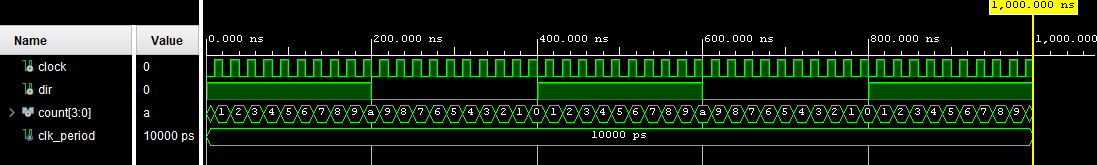
\includegraphics[width=0.75\textwidth]{resource/sim1.PNG}
        \end{center}
        Over a 1000ns simulation period, seen above, we can confirm that the counter incrementing per clk cycle, steps are even has overflows/resets correctly.
        \subsubsection*{Implement and Program}
        To run the implementation and prepare for writing the bitstream the package pins must be selected in I/O planning. The direction was mapped to a switch, each bit of the output to an LED and connecting the clk.

        One hiccup was the I/O std was initially on default, but displayed the correct value. This causes failure unless it was reselected.

        Once this was completed, the schematics and device can be viewed. When connecting the board via USB the board can be written to with a generated bitstream.

        \subsection{Part 2 : Slow it down}
        Visually the progression of the LED count is unreadable due to speed. To slow the display down, the internal count signal was increased to a 28bit vector incrementing at the same speed, but outputting the most significant 4 bits (LSB @ 5HZ).

        \subsection{Part 3 : 7-seg and FLASH}
        The binary output of the counter is hard to directly read from the LED, so we can use the 7-segment on the board to display the encoded character. This was done with a seperate decoder module that translated the 4bit binary to a 7 bit binary coded decimal fit for sending to the displays. While this is simple in concept, in the lab there was lots of opportunity to mistype and this caused multiple errors. 


\section{Questions}

\begin{enumerate}
        \item We are using the Xilinx Artix 7 FPGA (on the NexysDDR board) and has 324 pins (ie the defined package of the chip). 
        \item The onboard clock runs a 100Mhz crystal oscillator
        \item 100Mhz / 2\^24 = 5.96046448 hertz, assuming a flip per clk
        \item 100Mhz / 2\^15 = 3.05175781 kilohertz
        \item This line links the value of the internal signal that represents the current counter value the the count output of the module.
        \item A testbench defines a testing procedure for use in simulation to debug and confirm the behaviour of the code.
\end{enumerate}

\end{preview}
\end{document}